\documentclass[onecolumn, draftclsnofoot,10pt, compsoc]{IEEEtran}
\usepackage{graphicx}
\usepackage{url}
\usepackage{svg}
\usepackage{setspace}
\usepackage{float}
\usepackage{longtable}
\usepackage{pgfgantt}

\usepackage{geometry}
\geometry{textheight=9.5in, textwidth=7in}


\def \subparagraph {.}

\usepackage{titlesec}
\usepackage{hyperref}

\titleclass{\threesection}{straight}[\subsection]
\titleclass{\foursection}{straight}[\subsection]

\newcounter{threesection}[subsubsection]
\newcounter{foursection}[threesection]

\renewcommand\thethreesection{\thesubsubsection.\arabic{threesection}}
\renewcommand\thefoursection{\thethreesection.\arabic{foursection}}

\renewcommand\theparagraph{\thethreesection.\arabic{paragraph}}
\renewcommand\theparagraph{\thefoursection.\arabic{paragraph}}

\titleformat{\threesection}
  {\normalfont\normalsize\bfseries}{\thethreesection}{1em}{}
\titlespacing*{\threesection}
{0pt}{3.25ex plus 1ex minus .2ex}{1.5ex plus .2ex}

\titleformat{\foursection}
  {\normalfont\normalsize\bfseries}{\thefoursection}{1em}{}
\titlespacing*{\foursection}
{0pt}{3.25ex plus 1ex minus .2ex}{1.5ex plus .2ex}


\makeatletter
\renewcommand\paragraph{\@startsection{paragraph}{6}{\z@}%
  {3.25ex \@plus1ex \@minus.2ex}%
  {-1em}%
  {\normalfont\normalsize\bfseries}}
\renewcommand\subparagraph{\@startsection{subparagraph}{7}{\parindent}%
  {3.25ex \@plus1ex \@minus .2ex}%
  {-1em}%
  {\normalfont\normalsize\bfseries}}
\def\toclevel@threesection{4}
\def\toclevel@foursection{5}
\def\toclevel@paragraph{6}
\def\toclevel@paragraph{7}
\def\l@threesection{\@dottedtocline{4}{7em}{4em}}
\def\l@foursection{\@dottedtocline{5}{10em}{5em}}
\def\l@paragraph{\@dottedtocline{6}{14em}{6em}}
\def\l@subparagraph{\@dottedtocline{7}{19em}{7em}}
\makeatother

\setcounter{secnumdepth}{4}
\setcounter{tocdepth}{4}
\setcounter{secnumdepth}{5}
\setcounter{tocdepth}{5}


% 1. Fill in these details
\def \CapstoneTeamName{			PolyVox}
\def \CapstoneTeamNumber{		66}
\def \GroupMemberOne{			Chris Bakkom}
\def \GroupMemberTwo{			Richard Cunard}
\def \GroupMemberThree{			Braxton Cuneo}
\def \CapstoneProjectName{		3D Virtual Reality Painting}
\def \CapstoneSponsorCompany{		EECS}
\def \CapstoneSponsorPersonOne{		Dr. Kirsten Winters}
\def \CapstoneSponsorPersonTwo{		Dr. Mike Bailey}

% 2. Uncomment the appropriate line below so that the document type works
\def \DocType{		%Problem Statement
				%Requirements Document
				%Technology Review
				Software Design Description (Draft 1/5/2018)
				%Progress Report
				}
			
\newcommand{\NameSigPair}[1]{\par
\makebox[2.75in][r]{#1} \hfil 	\makebox[3.25in]{\makebox[2.25in]{\hrulefill} \hfill		\makebox[.75in]{\hrulefill}}
\par\vspace{-12pt} \textit{\tiny\noindent
\makebox[2.75in]{} \hfil		\makebox[3.25in]{\makebox[2.25in][r]{Signature} \hfill	\makebox[.75in][r]{Date}}}}
% 3. If the document is not to be signed, uncomment the RENEWcommand below
%\renewcommand{\NameSigPair}[1]{#1}

%%%%%%%%%%%%%%%%%%%%%%%%%%%%%%%%%%%%%%%
\begin{document}
\begin{titlepage}
    \pagenumbering{gobble}
    \begin{singlespace}
    	
\includegraphics[height=4cm]{coe_v_spot1}
        \hfill 
        % 4. If you have a logo, use this includegraphics command to put it on the coversheet.
        %\includegraphics[height=4cm]{CompanyLogo}   
        \par\vspace{.2in}
        \centering
        \scshape{
            \huge CS Capstone \DocType \par
            {\large\today}\par
            \vspace{.5in}
            \textbf{\Huge\CapstoneProjectName}\par
            \vfill
            {\large Prepared for}\par
            \Huge \CapstoneSponsorCompany\par
            \vspace{5pt}
            {\Large\NameSigPair{\CapstoneSponsorPersonOne}\par}
	    {\Large\NameSigPair{\CapstoneSponsorPersonTwo}\par}
            {\large Prepared by }\par
            Group\CapstoneTeamNumber\par
            % 5. comment out the line below this one if you do not wish to name your team
            \CapstoneTeamName\par 
            \vspace{5pt}
            {\Large
                \NameSigPair{\GroupMemberOne}\par
                \NameSigPair{\GroupMemberTwo}\par
                \NameSigPair{\GroupMemberThree}\par
            }
            \vspace{20pt}
        }
        \begin{abstract}
        % 6. Fill in your abstract    
The following is the design document for the program PolyVox, a virtual reality based three-dimensional art program. This document outlines the goals, requirements, and design decisions for the development of the program. These factors are based on the needs expressed by the project stakeholders, which are specified and addressed within the document.
        \end{abstract}     
    \end{singlespace}
\end{titlepage}
\newpage
\pagenumbering{arabic}
\tableofcontents
% 7. uncomment this (if applicable). Consider adding a page break.
%\listoffigures
%\listoftables
\clearpage

% 8. now you write!
\section{Introduction}
\subsection{Purpose}
This Software Design Description (SDD) specifies the design plan for the VR based 3D art program PolyVox. This document expands upon the content of the PolyVox Software Requirements Specifications (SRS), and specifies how the elements of the SRS are incorporated into the program. Additionally, this document addresses the design concerns of the project stakeholders, and how these concerns will be handled in the design. 
\subsection{Scope}
This document describes the structure of PolyVox and the implementation of its individual components. This document assumes that any reader is already familiar with the PolyVox SRS and the project as a whole. This document also includes details of elements as of yet not detailed in previous documentation, and provides context as necessary. 
\subsection{Intended Audience}
This document details the technical design of the PolyVox application, and, as such, is intended for readers with knowledge of programming and software development methods. 
\section{Glossary}
\begin{longtable}{ | l | p{12cm} | }
 \hline			
AR & Augmented Reality; The practice of producing a synthetic overlay interface that displays and dynamically interacts with the physical world around the user. \\ \hline 
Attribute & A class or value representable as one or more integers or floating point numbers  \\ \hline
Attribute datum & A specific instance of an attribute  \\ \hline
Color & A set of four attribute data, all represented by a floating point value, corresponding to red, green, and blue color channels, as well as an alpha (transparency) channel.  \\ \hline
CPU & Central Processing Unit; The component of the computer that runs and operates programs, and performs the necessary computations to do so.  \\ \hline
Framerate & The reciprocal of time between each temporally consecutive instance of a new image rendered by PolyVox being displayed to the user, measured as frames per second (fps). \\ \hline 
Grid &  Specifically, a finite three dimensional cartesian regular grid which is oriented relative to a three-dimensional origin by a transformation representable by a four-by-four matrix. \\ \hline
GPU & Graphics Processing Unit; a processor specifically designed to perform the computations used to render three-dimensional computer graphics.  \\ \hline
HMD & Head Mounted Display; A wearable display system placed over the user’s head and face with a display placed directly in front of the user’s eyes. The HMD also tracks the user’s head movements and sends position and orientation data to the program.  \\ \hline
Interchange & The program native to the CPU which is in charge of managing user interaction with the voxel state via Yggdrasil as well as maintaining CPU-side resources. \\ \hline
Latency & The measure of time between a user manipulating the devices they are interfacing with and the effects of these manipulations being displayed by the output of these interfacing devices. \\ \hline
Motion Control & The practice of manipulating devices which measure and convey to a computer their position and orientation relative to a reference point.  \\ \hline
Resolution & The number of columns and rows of pixels used in a display. In the case of  a VR headset, resolution is the number of columns and rows of pixels visible to one eye using the headset. \\ \hline
SVO & Sparse Voxel Octree; A technique used in ray tracing for voxels. Individual voxels are subdivided into octants, and the system determines which, if any, octants within a view are unneeded to render a complete image. If an octant is determined to be unnecessary, the system skips any rendering computations that would have otherwise been performed on it.\\ \hline
Virtual Reality & The practice of placing a display in front of each eye of an individual and displaying images for each eye which, through binocular vision, convey, to the individual looking into said displays, a scene with the illusion of depth.  \\ \hline
Voxel & An element of a 3D grid with an associated set of attribute data including at least one instance of color.  \\ \hline
Voxel State & The state of every instance of a geometric element explicitly represented by PolyVox during a given instant. This includes the transformation of each particular geometric element, the size of each geometric element along each of its three axes, and the states of all attribute data present in each voxel of each geometric element. \\ \hline
Yggdrasil & A collection of GPU programs which collectively manage the voxel state, including updating the data represented within and maintaining the associated resources on the GPU. These programs are called by the Interchange. \\ \hline
\end{longtable}

\subsection{References}
\bibliographystyle{IEEEtran}
\bibliography{Bibliography}{}

\section{Stakeholders}

\subsection{Dr. Mike Bailey}
Dr. Bailey was brought onto the project after being approached by Dr. Kirsten Winters, who inquired about designing a three-dimensional art program in VR. Dr. Bailey's primary stake in the project is the development of VR and graphical technology, with less concern for specific feature sets. His primary design concern is development of a stable and sufficiently robust graphics engine compatible with VR.
\subsection{Dr. Kirsten Winters}
Dr. Winters is responsible for the inception of the program, and brought the concept of a 3D art program to Dr. Mike Bailey. Her initial vision of the project is, by intention, rather open. As such, her main design concerns are higher-level functionality, such as the general ability to create three-dimensional geometry using motion controls, as well as maintaining sufficient program optimization to ensure a comfortable user experience.
\subsection{Intel}
In recent years, Intel has been supporting the development of VR and AR applications, going as far as forming a VR-centric department, the Intel VR Center of Excellence, in an effort to push VR into mainstream popularity. With this goal in mind, Raj and Bryan Pawlowski of Intel have agreed to aid the project and supply resources, with the intent of producing a viable VR product. Given these factors, Intel’s primary design concerns are focused around ease of use for users. These include program stability, accuracy of motion controls, functioning user interface, and a sufficient feature set, as well as comfortable user experience. 
\subsection{Development Team}
In addition to the project clients, the development team has a stake in the success of the project. As with all clients and the OSU school of EECS, all team members will receive equal, non-exclusive rights to the ownership of the program. As such the development team has an interest in developing a powerful and functional toolset for the program. With that in mind, the development team’s primary design concerns are maintaining program stability, flexibility of execution, and ease of extension.

\section{Design Views}


\subsection{Components of the User Interface}

While the premise of PolyVox, a 3D painting program, is a somewhat simple idea, there are several practical concerns that need to be addressed regarding how such a program should be designed with respect to artist flexibility as well as system performance. With respect to the user’s experience of the environment, the components of PolyVox fall under two broad categories, blocks and tools. Blocks simply act as a container for the geometry a user writes into the virtual space, and may be switched between several states to change how their contents interact with the rendering and tool programs of Yggdrasil. Tools, meanwhile, are what users use to alter the Voxel State, and are classified as either voxel tools or block tools. Voxel tools affect the content of whatever is considered the selected block whereas block tools affect the nature of the selected block itself, including size, position, and rotation.

What the user sweeps through space when they move their brush is, in essence, a box. This box is described by a four-by-four matrix, which encodes where the bounds of the box are in 3D space, given that the box is a cube of side length two centered at the origin which has been multiplied by that matrix. Various other attributes, such as stroke weight, are associated with the tool during its operation. More about the specific data associated with the tool tip and how it is used to achieve the effects described below will be included in the “How Tools Work” section.

\subsection{Block Tools}

\subsubsection{The Creation Tool}

The creation tool, as the name implies, creates a new block in the Voxel State and maps it into the currently selected block. Should no block be selected, the block created by the tool is mapped into the root block. The bounds of this block are equal the bounds of the tool tip at the time of creation.

The type of block produced can either by a standard block or a copy-on-write (COW) block. By default, a completely empty standard block is produced. If the user specifies with the focus block that they are copying a different block, then the type and content of the block matches that of the block being copied. The user may also choose to make a COW block out of a standard block, turning the standard block into a canon block. More about the distinction between a standard, canon, and COW block is discussed later.

\subsubsection{The Deletion Tool}

The deletion tool, quite simply, removes the currently selected block and frees all data associated only with that block. Should the block be a COW block, the underlying data is not freed unless it is the last block referencing the underlying SVO head. Additionally, all blocks mapped into the selected block will recursively undergo deletion as well.

\subsubsection{The Mapping Tool}

The movement tool unmaps the currently focused block from its original location in its mapping black and remaps to the bounds specified by the tool tip in the currently selected block. Should no block be selected, the currently focused block is mapped into the root block.

\subsubsection{The Selection Tool}

The selection tool performs a trace along a path starting at the tool tip and extending in the direction to tool is pointing, searching for blocks. The selection tool looks for the Wth block along this path, where W is the current value of the tools weight, rounded down to the nearest integer. Should this Wth block be found, it becomes the new selected block and the previously selected block is no longer selected. Should this block not actually be found, or if this block is the root block, no blocks are considered selected. Additionally, should the user specify that the block found is to be marked as the focus block, the same process occurs, but with the application of the focus state instead. 

\subsubsection{The Hide/Unhide Tool}

The hide/unhide tool simply sets the state of the block to be hidden if it currently is hidden and vice versa.

\subsubsection{The Save Tool}

The save tool saves the currently focused block to a file specified by the user. Should no block be focused, the root block is saved in the filename associated with the currently open Voxel State unless it does not exist or is otherwise specified.



\subsection{Voxel Tools}

The categories of tool discussed below are not single instances of voxel tools, but different classes of voxel tool, under which practically limitless permutations can exist. Unlike block tools, the user base of PolyVox likely requires a variety of specialized voxel tools in order to meet particular needs. However, these tools can be segmented into classes which embody specific behaviors that all members would have in common. These common behaviors, in turn, will be developed into code templates and built-in variables that both the developers and users of PolyVox may use to create custom tools without the hassle of setting up the necessary boilerplate code.

\subsubsection{Basic Tools}

Basic voxel tools are perhaps the most limited of the voxel tool classes, but this comes with reduced computational cost in the supporting code. The injected code can determine two things regarding the end state of the block being affected, how deep the SVO of the block is at any given location and the data local to the affected leaf nodes. When affecting the data of a specific node, only the pre-existing data of the current node is readily accessible.

\subsubsection{Adjacency Tools}

There are some processes, such as kernel convolution, which necessarily require knowledge of neighboring voxels in order to be possible. Unfortunately, this necessitates that the affected region of space is all at a uniform level of depth and that the data of these voxels are stored somewhere that can be accessed across threads. Taking use of image reads and writes, threads affecting the data of any given node can access the data of any other node in the grid of affected voxels prior to determining its local data.

\subsubsection{Fill Tools}

Some processes, such as a bucket fill algorithm, require the iterative traversal of voxels in an expanding body. Given the wildly varying nature of how long such a process can take, as well as the fact that fill-based tools do not rely upon a “painter’s stroke” to guide form, the user’s tool is disabled for the remainder of the fill operation, with the exception of an option to cancel the fill. To keep frame rate high, the number of nodes that may be expanded into by a fill operation is capped per-frame and the remainder of the fill operation is delegated to the subsequent frames.


\subsection{Block Types}

\subsubsection{Standard Blocks}

As the name implies, standard blocks act as the default for how Yggdrasil treats blocks. Standard blocks may be traced into by the rendering programs of Yggdrasil and may contain mappings into other blocks. Furthermore, voxel tools may actively manipulate the contents of a standard block, so long as that block is selected. Lastly, when a standard block is copied, the resulting block is a deep copy of the original block’s data, and so writes to either block should not affect the content of the other.

\subsubsection{Copy on Write (COW) Blocks}

COW blocks serve as a method of producing identical copies of an object with less overhead than making a deep copy. All COW blocks reference a block as its canonical content, a canon block, and traces into a COW block are redirected to its canon block. Additionally, if a voxel tool attempts to write into a COW block or a mapping attempt is made on the block, the initial tool attempt is denied and the block is converted to a standard block with a deep copy of its canon block. For obvious reasons, the more data that resides in the canon block of a COW block, the longer it takes to perform a deep copy. Copies of a COW block, however, simply yield COW blocks that refer to the same canon block.

\subsubsection{Canon Blocks}

As stated above, canon blocks act as the container for data referred to by COW blocks. Canon blocks operate like standard blocks with the exception that may not be mapped anywhere other than the root block and may not be deleted until all of their associated COW blocks are deleted. Copy attempts on a canon block simply yield a standard block with a deep copy of the canon block, so the data contained within a canon block may only be referred to by a single canon block. This is simply done to simplify the matters of managing canon blocks. If a canon block could be mapped into another block and that block was deleted, the deletion would either have to abort or delete the canon block, potentially leaving COW blocks with hanging references.

\subsubsection{Hidden Blocks}

As with most artistic programs, it is convenient for creators to remove specific content from their view so that a particular component of their work may be viewed more clearly. To these ends, any of the above blocks may, additionally, be classified as a hidden block. Hidden blocks are simply marked by Yggdrasil such that rendering passes and tools other than the select and hide/unhide button know to ignore them. 

\subsubsection{The Selected Block and Focus Block}

Any of the blocks mentioned above can be classified as the selected block or the focus block. At any given time, there can be at most one selected and focus block, and they may not be the same block. These classifications act as a signal to Yggdrasil what blocks are being operated upon during an operation. Furthermore, whenever a block is made a selected or focus block, a block is mapped around that block which provides color-coded outlines of that block. This allows the user to discern which block is the focus block and which is the selected block.

The need for both a selected and focus block comes from the fact that the user must be able to control which blocks are involved in an operation. In general, the selected block is the block which is affected by an operation, whereas the focus block is used as an argument in that operation. For instance, the mapping tool maps the focus block into the selected block.

\subsubsection{The Root Block}

For the sake of organizing the data within the Voxel State all user-created blocks are held within a root block. This arrangement simplifies several aspects of how PolyVox operates. First, this enables Yggdrasil programs to quickly test whether or not blocks in the virtual environment are overlapping, which is important for rendering the environment with realistic transparency. Secondly, it establishes a universal starting point for ray traces and a quick means of detecting when ray traces collide with blocks. Thirdly, it adds versatility to the program by enabling the user to apply some block manipulating tools to the virtual environment as a whole. Of course, the root block will be actively ignored by the deletion and hiding tools, as irreversibly destroying the entire virtual environment or rendering it invisible is not a commonly required action and can be catastrophic if accidentally performed. Lastly, for obvious reasons, only one block may be of the root block type and may not transition to any other type. Likewise, no non-root block may ever transition into being a root block.




\subsection{Components of the Voxel State}

The Voxel State is the representation of the virtual environment the user is interacting with, as stored and organized within the GPU. The primary design concerns pertaining to the Voxel State are efficiency of space, speed of manipulation, and versatility. 

The overall system is intended for an art program, which implies extreme freedom of manipulation. As such, one cannot assume a maximum limit upon the amount of data required to represent what the user is creating. Therefore, the best way to meet the potential memory demands of the user is to be efficient with whatever amount of memory is at the disposal of the GPU. Additionally, the high refresh rate expected from PolyVox necessitates fast parallel access to the data within the Voxel Sate. The speed offered by a GPU is limited if operations require serial access to data. Thus, representing data in a distributed fashion that allows multiple agents to operate on different data at the same time is crucial. Lastly, given that the nature of this project is exploratory, little is known about the specific methods which would be applied to PolyVox as a whole. In order to best meet such uncertainty, versatility in use must be incorporated into how the Voxel State represents geometry.


\subsubsection{Nodes and their Usage}

\threesection{Overview}

The basic unit of memory in the Voxel State is the node. Nodes are contiguous sections of 64 bytes in the DataBuffer. Nodes are primarily used to store the data that encodes voxels in the Voxel State, although they are used to store other data too, including transformation matrices, task data, COW block identification, and face lighting data.


\threesection{Nodes as Voxels}

In terms of a C struct, a node used to encode a voxel has the following data layout:


\begin{verbatim}
        struct voxel {
                uint32_t meta;
                uint32_t surface;
                uint32_t mappingList;
                uint32_t faceLightingIndex;
                uint32_t attributes[4];
                uint32_t children[8];
        };
\end{verbatim}


\foursection{Meta Usage} The meta field acts as storage for several flags that help to streamline the process of working with nodes.The least significant bit of this field is used to encode whether or not the node or any of its children emit light. This piece of data is used for certain types of voxel cone traces. The remaining bits are left for potential future use in encoding different types of voxels.

\foursection{Attribute Usage}

While the meta field has extra space to indicate different types of voxel, there currently is only one type. This standard voxel type encodes eight attributes, distributed across the four attribute fields through the use of GLSL’s built-in floating point packing function. The first four attributes encoded are three color channel values and an alpha value. The usage of these attributes is standard with common practices. The second four values are roughness, index of refraction (IOR), scatter, and glow. Roughness and IOR correspond with common usage in physically based rendering (PBR), where roughness corresponds to how much a surface scatters light during a bounce and IOR corresponds to how the incident angle of light affects what proportion of light is reflected or refracted. Scatter corresponds to how readily light is internally scattered through the material the voxel represents. Lastly, glow corresponds to the light output of the material per unit volume. For the sake of simplicity, it is assumed that the color channels of the output light are directly proportional to the material’s color channel.

\foursection{Surface Usage}

In spite of being represented within 4 bytes, the surface attribute encodes 4 floating point numbers via the GLSL-native floating point number packing, which allows for the first eight bytes of the mantissa of four different normalized floating point numbers to be packed into and out of a uint from a vec4. The first three components of this vec4 represent the normal of the surface contained within the voxel and the fourth component represents the offset of this surface from the center of the voxel (along the normal). Should the magnitude of a surface field  normal be zero, this indicates that the surface field is not valid for representing a surface.
A points position relative to the surface (whether it is inside or outside of the surface, and by how much) can be calculated by mapping the point to the space relative to the voxel, performing a dot product between the mapped point and the surface normal , then subtracting the result by the fourth component of the surface field. The position mapping is translating and scaling the position’s coordinates such the relative bounds of the cube fill a 2x2x2, axis aligned cube centered at the origin. This mapping means that the surface field can work regardless of the actual scale of the voxel. From there, the dot product and subtraction establishes the point’s position relative to the surface, such that positions greater than zero are above the surface and positions less than or equal to zero are below the surface. 

\foursection{Face Lighting Index Usage}

While taking the average of voxel data to calculate parent voxel data works with children of comparable content, as the difference in transparency and illumination glows, it can cause light and transparency to apparently “bleed” into regions of space which should display little to none of either. For instance, if a thin plain of opaque voxels were made and then brought further from the camera, it would appear to grow more transparent with distance. In order to remove these artifacts, information about how the voxel appears from each side is necessary. This is problematic because, even with minimal representation, another node needs to be allocated in order to store all of this data. The index to this additional node is stored in the face lighting index field.

This being said, such additional storage is not necessary for all nodes. Leaf nodes with no cached children must, by their very nature, represent a homogeneous region of space and thus does not a face lighting node. Additionally, voxels that have children with relatively similar properties create negligible artifacts. Lastly, only voxels with children that exceed the depth limit of tracing or are cached outside the GPU can create these artifacts. Thus, by frequently performing voxel culling and creating face lighting nodes only for voxels containing widely varying data, the additional memory overhead expected should be kept to a minimum.


\foursection{Child Usage}

The position of each child field in a node is directly associated with the position of that child in its parent. For every child field in a node, that field’s position in the list of child fields encodes which octant of the node it occupies. Should the first bit of this position, when represented as an unsigned integer, be set, the corresponding child is on the positive X half of its parent. This holds true for the second and third bits of this positional value in the Y and Z dimensions, respectively. 

The value of a child field indicates several things about that child. Should the first 31 bits of the field be set, the child is considered null. Being null does not necessarily mean that the child referenced does not exist, as it may be held in backing storage to reduce memory usage. Should this be the case, the 32nd bit of the field is set.

\foursection{Mapping List Usage}

As stated previously, blocks can be “mapped” into other blocks. Mapping, in this context, refers to leaving a reference to one block within one or more voxels in another block. These references come with the index of the mapped block’s SVO in the Head Buffer and an identification number representing whether or not the mapped block is a COW block and, if so, which one. Such mapping lists allow traces to trace through mapped blocks as if they actually were contained in the mapping block. Mapped blocks each have an associated transform local to their mapping block and are only included in specific voxels of the mapping block. Specifically blocks are only included in the mapping list at a depth with the smallest voxels that still exceed the minimum dimension of the block. Furthermore, references to a mapped block are only included in the voxels of the mapping block which contain the bounds of the mapped block. Lastly, the ordering of blocks in a mapping list is determined by the precedence of the block, where blocks with a higher precedence are closer to the beginning of the list. These restrictions ensure that ray traces into blocks are only made when rays are in a close vicinity to the block’s actual location and are made in proper order, by precedent.

 

\threesection{Nodes as Face Lighting}

The data layout of a face lighting node, in terms of a C struct, is this:

\begin{verbatim}
        struct faceLighting {
                uint32_t color [6];
                uint32_t light [6];
                uint32_t misc  [4];
        };
\end{verbatim}

In essence, the appearance of a voxel for each face is represented in two lists, one for the color of the voxel and one for the light emitted by the voxel. The ordering of faces in this list are as follows: -X, +X, -Y, +Y, -Z, +Z. The remaining space in this node, as of this time, has no use.

A face lighting node may be constructed from a node’s children by iterating through each face of the voxel and calculating the average color and light output along the normal of that face. This is done by iterating through each pair of children aligned along this axis and using the alpha of the children nearer the face to perform a weighted average between the properties of the nearer and further children. From their, the four resulting values are averaged, and the process is repeated for the rest of the nodes.

\threesection{Nodes as Transformation Matrices}

Being exactly the size of a transformation matrix, nodes are sometimes used to store a mat4. Particularly, the transformation matrices of all blocks are stored in a node.

\threesection{Nodes as Tasks}

Depending upon the program running, the content of a task node can vary. However, there are two common elements to all task nodes; The first 4 bytes of a task node are a pointer to the task’s parent node and the second 4 bytes of a task node are a count of how many child tasks the task node has. The precise usage of these fields is explained in later sections.


\subsubsection{The Data Buffer} 

As stated previously, all nodes in the Voxel State are contained within the Data Buffer. In fact, the Data Buffer consists only of nodes and serves little other purpose than acting as a large section of memory. The data that helps Yggdrasil interpret and manipulate the Voxel State is present in other buffers, namely the Block, Heap, Task, and Exchange buffers. References to specific nodes are stored as their index in the Data Buffer, and shall be referred to simply as node indexes.

\subsubsection{The Block Buffer}

The Block Buffer contains the properties of all blocks in the Voxel State. These properties include a blocks matrix transform, parent block, reference count, type, and root. The matrix transform of a block is simply a four-by-four matrix encoding the bounds of the block much in the same way a four-by-four matrix encodes the bounds of a tool tip. The parent block of a node is an unsigned integer equal to the index of a block, otherwise known as a block ID. A parent block property, in particular, references the block which contains a block by mapping. The reference count of a block is zero, unless the block is a canon block, in which case the reference count is the number of COW blocks currently using that canon block as a reference. Meanwhile, the type of a Block Buffer element is just that, an enumeration describing which type of block that specific element represents. Lastly, the root of a block is the index of the root node of the SVO containing the block's data.


\subsubsection{The Heap Buffer}

The Heap Buffer contains a series of node indexes and integer counts, where each index is followed by a count in an alternating fashion. Each of these pairs represent a linked list of unused nodes in the Data Buffer, where the index of a pair references the head of the list and the count stores the length of the list.

At the startup of PolyVox, the lists of the HeapBuffer are initialized with linked lists containing all of the memory of the Data Buffer, as no data is being used yet. These lists are distributed evenly such that no pair of lists in the Heap Buffer can vary in length by more than one.

During execution, each thread in a Yggdrasil program is assigned a set of three contiguous pairs from the Heap Buffer. The first element of each triplet is always kept filled with a list, though the list occupying that spot may vary across time. The remaining two lists are used for allocating and freeing memory, where nodes are removed from lists of longer length and nodes are freed by placing them into the list of lower length. This generally results in the lists being of equal size. Additionally, after some period of execution, a program may perform a swap between the lists of different triplets, which generally results in the number of nodes available in each triplet becoming more level.

This setup enables Yggdrasil programs to perform non-blocking constant-time memory allocation, which offers a significant boost in memory operation speeds, compared to the alternative.


\subsubsection{The Task Buffer}

The Task Buffer is identical to the Heap Buffer in size, form, and function with the exception of one detail. Whereas the Heap Buffer stores free memory for programs to retrieve, the Task Buffer stores tasks for programs to perform. Regardless of this discrepancy, the reasoning is the same: resources distributed more evenly across threads promotes better performance. In the case of tasks, more evenly distributed tasks leads to fewer threads needlessly idling.


\subsubsection{The Exchange Buffer}

The Exchange Buffer contains either requests for subtrees of SVOs or the SVO subtrees, themselves. Both subtree requests and actual subtrees come with a set of information qualifying which specific subtrees are being referred to. This includes the ID of the subtree’s containing block, the depth of the subtree’s root in the block, and the position of the subtree’s root in the block. In the Exchange buffer, such identifying information occupies three contiguous elements in that order.

Immediately after this identifying data, requests have only one additional component, the height of the requested tree. This allows the GPU to request only the layers of an SVO it needs, which is important for maintaining performance.

The identifying data of subtrees resident on the Exchange Buffer are followed by an integer value and an array of nodes. The integer value simply denotes the number of nodes in this array, whereas the array is a left-order traversal of the encoded tree. To prevent ambiguity, a light node is considered to be left of the content of the node’s mapping list, which is left of the node’s children.

The data for subtree requests are all placed into a contiguous section starting at the third element of the Exchange Buffer. Immediately following this array is another array, containing one element for each tree present in the Exchange Buffer, where he nth element of this array stores the starting index of the nth tree. The data for these trees, in the presented order, is placed immediately after this array. Finally, encoding the lengths of the request array and the tree index array are the first and second elements of the Exchange buffer.


\subsection{Components of the Graphics Engine (Yggdrasil)}

Yggdrasil, named for the cosmic world tree of Norse mythology, is the framework of GPU-native programs that are in charge of managing and rendering the Voxel State for PolyVox. As with the Voxel State, efficiency of memory usage as well as speed are strong design concerns. For this reason, reducing function runtime per input as well as memory footprint required for operations is key.


\subsection{Tasks}

One of the biggest challenges of this project is that it deals with a distinctly non-uniform data structure that can be potentially so large that maintaining precise statistics about it as it changes would be impractical. GPUs, by their very nature, work best with performing the same task in parallel as part of massive groups. In fact, at the very outset of a compute shader, the number of work items used is essentially set in stone. Thus, it is problematic to try to match the number of work items with the units of work that are to be accomplished because it is not known how many of these units of work there are. Additionally, some of these units of work need to be performed in order to determine whether other units of work should be performed, and the number of units of work that a given unit can produce is difficult to predict.

This may bring some to wonder why it is not better to apply a CPU to this problem rather than a GPU. The answer is that, aside from this variability regarding how many units of work are to be performed, these tasks lend themselves heavily to the massively parallel capabilities of a GPU. To help bridge this gap, PolyVox will keep track of what units of work need to be performed as tasks.

As described in previous sections, the data that encodes a task is stored in a repurposed node data structure. During the outset of any of its programs,
Yggdrasil allocates and fills nodes with data corresponding to the initial set of tasks that need to be performed for whatever it needs to accomplish. During the processing of a given task, several subsequent tasks may need to be performed to complete the work of that initial task. These subsequent tasks, as they are found necessary, each have a node allocated and filled with data describing what needs to be done. After this initial allocation is done, the new tasks are pushed into that work item’s task list. Once a work group finishes a round of tasks, it performs a simple balancing operation across each work item’s task list, then each work item takes the top task in its task list and the process starts over again.

Along the way, some work groups may become starved of tasks while other work groups are overburdened. An issue in addressing these cases is the delay required to communicate between work groups. Should work groups communicate frequently with one-another, tasks will be distributed more evenly but the overall amount of time required to process a number of tasks decreases. To minimize this, a few simple heuristics are used to ensure balancing across groups occurs only when necessary:

Every work group has two shared unsigned integer variables, called Starved and Fed, respectively. Additionally, there are two global variables called Glob\_Starved and Glob\_Fed.  After a number of task completion cycles are performed in a work group, every work item in that work group atomically increments Starved if they have no tasks in their task list or Fed if they have tasks in their task list. Should the ratio of Starved and Fed exceed some threshold, the work group atomically increments Glob\_Starved, otherwise Glob\_Fed, then sets Starved and Fed to zero. Should either the former or new ratio of Glob\_Starved and Glob\_Fed exceed some threshold, the work group performs a task list balance operation with some of its fellow work groups and sets both Glob\_Starved and Glob\_Fed to zero.

One problem that arises from such a dynamic, distributed system is that it can be difficult to determine when a program is done. To resolve this, tasks have an established hierarchy of execution. Whenever the processing of a task causes another task to be created, this new task has its parent field set to the index of the original task and the ChildCount field of the original task is atomically incremented. When a task is complete, it atomically decrements the ChildCount field of its parent and, if the resulting value is zero, decrements the ChildCount of that task’s parent, continuing the process until it performs a decrement that does not result in a zero or it causes the root task’s ChildCount to hit zero. The root task is an additional task that is allocated at the beginning of a Yggdrasil shader invocation to act as a parent to all of the other tasks. Should it’s ChildCount hit zero, the work item processing the decrementation sets a global flag, signalling all work items to exit execution.


\subsection{Traversal and Task Ordering}

In Yggdrasils programs, with the exception of those involving VCTs, the processing of the Voxel State happens through a guided depth-first traversal of the entire area “of note” to the program. This is accomplished by a rather simple heuristic:

The root task analyzes the root node of the SVO being processed. Should further processing be needed in any of that root node’s children, a task is made and adopted by the current task for each of these children. This process occurs recursively. Should a task produce no children, it processes its node then terminates. Should it be the last child of its parent, the task performs further processing for the parent, if necessary, then terminates the parent.


\subsection{Tracing}

The various aspects and avenues of traversing through the SVOs of the Voxel State make performing a VCT a non-trivial process, particularly with regard to transparency. There could be any number of blocks overlapping a region of space, and a trace needs to be able to account for the contributions of each of these blocks to the value a trace returns as well as to the effects of each of these blocks on their neighbor’s lighting.

\subsubsection{Hits}

Before one can detail how VCT is performed in Yggdrasil, one must consider how the precedence and ordering of samples by VCTs is established. First, whenever a voxel is traced into, it first makes a determination of whether or not it “hit” anything in that voxel. Should the contents of the voxel be easy to represent as a plane, the surface attribute of that voxel may be used to make a collision check with that surface. This is done by checking if either the entrance or exit point of the ray in the voxel is the side of the surface opposite its normal. Should this be the case, the ray has hit. Additionally, should the contents of a voxel not be readily representable as a surface, it counts as a “hit” as well.

Establishing when a trace hits something is important insofar that, at any given moment in a particular SVO, a trace always considers itself to be traversing through some material. The default of this material, whenever a ray begins a trace, is a completely transparent substance. However, as soon as a ray hits in a voxel, this material is changed to whatever color is local to that voxel. From then on, the ray counts this color as the material it is traveling through until it either hits one of that voxel’s descendant nodes or traces beyond the confines of that voxel. Should the latter occur, the trace reverts its assumed material to that of the parent voxel. 

It should be noted that voxels with a valid surface field will not undergo hit detection using their surface field unless a trace is either at its depth limit or is attempting to trace through a null child of the voxel. Should this be the case, the trace must necessarily be at the highest resolution element either allowable or possible. This ensures that traces don’t register hits on surface fields that act as lower-resolution representations of a child’s surface field, which would cause problematic artifacts, inaccurate representations of the Voxel State, and unnecessary computational cost.

Hits, themselves, are calculated by normalizing the starting and ending positions of a trace through a voxel, performing a projection upon the surface normal, then using the projected positions to determine how far in or out of the surface the starting and ending positions are. Should both be on one side or the other, the full length of the trace through the voxel is used with the appropriate color to determine the effect upon the return value of the trace. Should the trace cross the surface, the ratio of the projected positions is used to determine what portion of the trace exists on each side of the surface and calculates  the effect upon the return value of the trace.

Return value calculations assume that an alpha of 0.5 halves the transmission of light through a voxel the size of the root block. Thus, for a voxel of size $2^{-X}$ with an alpha $A$, light transmission through the block is reduced by a factor of:

\begin{center}
$R = A^{2^{-X}}$
\end{center}

\subsubsection{SVO Traversal}

Disregarding traversing through mapped blocks, which is discussed below, the manner in which traces traverse an SVO is relatively simple. A trace through a single SVO is tracked with a stack that has a granularity of 16 bytes. Each chunk of 16 bytes in such a stack make up one vec3 and an unsigned integer. The unsigned integer indicates a specific voxel node in the Data Buffer, whereas the vec3 corresponds to the starting position of a trace through the voxel represented by the node. This starting position is transformed to a coordinate space local to the voxel, where the center of the voxel is the origin and the faces of the voxel are one unit distance away from the origin in whatever direction their normal is facing.

For any given SVO, a trace through that SVO begins with a single element on the trace’s stack. This element holds the index of the root voxel node of the SVO as well as the initial position of the trace relative to that root node. When iterating the trace forward, the trace’s work group first reads the top element of the stack and establishes the corresponding node and position as the active node and position of the trace’s state. Should the position of the trace fall outside of the voxel, the thread determines if the trace will ever intersect with the node, given its direction. If the test returns negative, the top element of the stack is removed and restarts the traversal process. Otherwise, the thread simply moves the trace along its direction of travel until it is inside the voxel. 

After this, the thread checks which octant of the node the trace is in and checks if the corresponding child field of the node is null. If this field is not null and the trace is not at its depth limit, the thread determines the position of the trace local to the coordinates of the child, stores this transformed position and index into the stack, then increments the trace’s depth value. If the corresponding child field is null, it calculates the lighting effects on the trace given the data local to the node. This includes surface hit detection, adding to the light values of the trace, and delegating child traces, should the trace not already be at its bounce or distance limit.

From there, the position of the trace is pushed along its direction of travel until it is out of its current octant and the traversal process begins again with whatever element is at the top of the stack. 

This process of adding to the local list repeats until the trace escapes from the bounds of the voxel, at which point the highest bit of the index most recently placed in the list is set, the depth value of the trace is incremented, and the contents of the list are pushed onto the stack in reverse order. After this the overall tracing process begins anew with the top element in the stack.

The traversal process may end in one of three ways. The potential gain in light accumulation left for a trace drops below a certain value, indicating that further tracing has negligible returns. Alternatively, the bounce or distance limit for a trace may be reached, leading to the trace stopping early to prevent further resource usage. Lastly, the trace may remove the remaining element on the stack, indicating that it has traced out of the SVO. 

\subsubsection{Mapped Blocks}

One of the biggest problems PolyVox faces is ensuring that users have freedom in expression, including the overlapping of multiple objects in the same space. This can be challenging, as it is difficult to determine adjacency between voxels, at least locally. Furthermore, organizing the data of overlapping voxels and determining order of processing through said voxels is non trivial.

To simplify matters, PolyVox will apply a number of rules. This includes the rule that all blocks not already mapped onto a block are mapped onto the Root block. This also includes the rule of block precedence, where every block has a unique ordinal number and traces into overlapping blocks perform tracing calculations in descending order of precedence. Lastly, this includes the rule that tracing calculations may only be performed over swaths of space where none of the traced blocks in an overlapping space transition into a new voxel. 

The first rule ensures that all blocks are reachable from a single block, either directly be being mapped into the root block, or indirectly by being included along a chain of mapping beginning at the root block. This means that ray traces beginning at the root block can reach all of the blocks in the Voxel State and hence can accurately represent that state visually.

The second rule ensures consistency of rendering. By asserting a hierarchy of precedence in tracing through blocks, the hierarchy can be exposed to the user such that they can have more control over the appearance of their work.

The last rule mainly exists as a matter of common sense. If a trace were to perform calculations for a swath of transparent material in one block that overlaps with the boundary between a transparent and opaque block, the result of the trace would not match with what common sense dictates.

To manage the simultaneous traversal of blocks, traces have a list in which they store references to each ray trace stack as well as an associated stack size, block ID, child count, and a reference to another list. All traces begin with a single-element list with the sole element corresponding to the root node. As a trace encounters mapped blocks in the root node, they are added to the root node’s list of mappings such that higher-precedent blocks appear sooner in the list. Furthermore, the executing thread begins traces for the blocks using their corresponding stacks. As mappings are found in these newly added traces, the lists corresponding to these traces accumulate their mappings. Then, as tracing in an element ceases, it and all of its children are freed from the structure.

This dynamic tree of mappings is what traces iterate over when performing their traversal operations, starting at the root and making a left order traversal of the tree, following the children of higher-priority blocks first before moving onto lower-priority blocks. With each traversal operation, the thread calculates the distance required for the currently operating traversal to reach a voxel boundary, and the current running minimum and second minimum are tracked. As per the third rule established for overlapping blocks, no traces may exceed this minimum metric until the block with the corresponding minimum distance has cleared such a distance. Thus, with each loop through the tree, all traces are advanced by this minimum and, as the minimum distance is crossed with its corresponding voxel, the second minimum distance is subtracted by the minimum distance and is established as the new minimum distance.

As overzealous and convoluted as this setup may seem, considering that one is managing a tree structure of potentially great size per trace and possibly slowing many traversals of a trace to a crawl to accommodate a few, more high-detail, traversals. For the former concern, one must consider that the vast majority of scenes produced by users will likely not have more than eight blocks overlapping one-another at any given point. For the latter concern, one must also consider that the majority of objects in the average scene are opaque and the majority of voxels representing empty space are larger than the average voxel. So, generally speaking, slowing traversals encountering less detail so that they keep pace with traversals over high-detail geometry generally prevents excess work from being done, as the voxels causing the slow down are likely to terminate the trace. Even operating under the assumption that overlapping traces in different blocks can be independently run and somehow “interleaved” into an accurate result later, it forces processing to occur over the sum of the distance required for all traversals. Meanwhile, the above solution bounds all traversals to travel the minimum distance required.



\subsection{The Programs of Yggdrasil}

\subsubsection{The Memory Manager}

Throughout the course of natural operation, Yggdrasil programs perform periodic balancing procedures to try to maintain the even distribution of resources. While these periodic balances may work well for a time, they are only designed to remove the most egregious imbalances. The Memory Manager serves to perform a more thorough balancing procedure upon the heap buffer set up future Yggdrasil calls for better performance.

\threesection{Parameters}

\textbf{ResourceSize} : an unsigned integer representing the size of the task and heap buffers.

\noindent \textbf{ShiftCount} : an unsigned integer representing how many times the linked lists of an individual heap are balanced before performing a swap.

\noindent \textbf{SwapCount} : an unsigned integer representing the total number of swapping operations.

\noindent \textbf{SwapStride} : an unsigned integer representing the bit offset used for the initial swapping operation.

\threesection{Operation}

The Memory Manager is mainly two nested loops, with the inner loop performing ShiftCount balancing operations upon individual heaps in the Heap Buffer and the outer loop performing SwapCount balancing operations between heaps in the Heap Buffer.

In the inner loop, heaps are balanced by first determining which of the node lists have a difference in length greater than one, such lists are considered imbalanced. For each pair of imbalanced lists, the Memory Manager moves up to ShiftCount nodes from the larger list to the smaller one, aborting early, should the lists become balanced.

In the outer loop, heaps are balanced by swapping list heads. Which heaps exchange list heads is determined by the SwapStride, where heap elements with indexes that are identical to one another except their SwapStride-th bit act as swapping partners. With each iteration of this outer loop, SwapStride is incremented and modulated by the base-2 log of Resource Size. This means that, assuming ResourceSize is an even power of 2, every heap element will be able to participate in a swap during any given iteration.

After these nested loops, the Memory Manager performs a reductive operation on the heaps, calculating the minimum and maximum list length throughout the Heap Buffer. The calculated minimum and maximum is then placed into the first and second element of the Exchange Buffer and the program is terminated.

\threesection{Usage}

For optimal results, the SwapStride of a Memory Manager execution should be equal to the sum of the SwapStride and SwapCount of the previous Memory Manager execution modulated by the base-2 log of ResourceSize. Additionally, the Memory Manager should be executed periodically throughout the operation of PolyVox, particularly after resource-intensive operations and during times of high memory use.

During times when the Memory Manager reports a higher range in list lengths, subsequent executions should increase both ShiftCount and SwapCount, although ShiftCount should generally be increased more quickly than SwapCount.


\subsubsection{The Tree Manager}

\threesection{Overview}

It is impractical to expect a GPU to hold all of the data a user could possibly generate in a 3D painting program. It is also unlikely that the user would require access to all of this data at once. To solve this, the Tree Manager acts as a method of loading and storing data in the Voxel State in accordance with the contribution of that data to what the user can see. 

\threesection{Parameters}

\noindent \textbf{Center} : a vec3 representing the location of the user in the virtual environment

\noindent \textbf{StartDepth} : an unsigned integer representing the deepest the Tree Manager should begin left-order searches for cullable and cached nodes.

\noindent \textbf{Dither} : an unsigned integer representing the proportion of the Voxel State that is checked by the Tree Manager, where the proportion is 2 -Dither.

\noindent \textbf{DitherStep} : an unsigned integer representing which step of a dithered management process the current program execution is.

\noindent \textbf{CullDepth} : an unsigned integer representing the lowest size of voxel that should be designated as “worth including” with the side length of such a sized voxel being 2 CullDepth times smaller than the side length of the root node of the root SVO. All voxels smaller than this will be considered to be in need of culling.

\noindent \textbf{DistanceFactor} : a floating point number representing how distance from the location indicated by Center will affect culling. Specifically, the effective value of CullDepth for a given voxel in the state will decrease with the log of its distance from Center multiplied by DistanceFactor.

\noindent \textbf{FaceLightingRange} : a unsigned integer representing how close a voxel qualifying for a face lighting node must be to culling before being given a face lighting node.

\noindent \textbf{ExchangeSize} : an unsigned integer representing how large the Exchange Buffer is.

\threesection{Operation}

The Tree Manager has two main stages of execution. The first of these stages is offloading any subtrees in the Exchange Buffer into the Voxel State. This is done by performing a traversal for each subtree to its location within its particular block and copying the contents of the subtree into the Voxel State along a left-order traversal, allocating nodes and copying data as necessary.

The second of these stages is placing cullable subtrees and subtree requests onto the Exchange Buffer. Subtrees valid for culling or retrieval are searched by a group of tasks, where each task begins its search is dependant upon the StartDepth, Dither, and DitherStep variables. When setting up these search tasks, each voxel of depth StartDepth or shallower is given a search task. Each of these search tasks delegate child search tasks based upon the value of Dither and DitherStep. Threads do this by iteratively traversing downwards, each time selecting the child field with the index equal to the first three bits of Dither Step then bitshifting DitherStep right by three bits. Once this traversal process has been repeated Dither times, the current voxel node of the thread is used as the beginning of its search.

The Tree Manager performs its searches by full left-order traversal of the subtrees rooted at each of the search task’s starting nodes. During this traversal, each time a thread encounters a new node, the depth is compared with the culling depth divided by the base-2 log of the voxel’s distance from the user. Should the depth be over the cull depth, the children of the node are checked for their most significant bit. If this bit is set for the field, it indicates that the child is cached by the CPU and will need retrieval. Thus, for every child found with this bit, space for a request is reserved in the Exchange Buffer, if possible. If the reservation is successful, the thread writes a request for that child with a tree height equivalent to remaining number of layers above the local cull depth.

If a search task begins to traverse below the local cull depth, it begins to track nine numbers. The first of these numbers is the lowest node depth it has backtracked through as part of its left order traversals after dropping below the culling depth. The remaining eight values are the number of nodes held by each of that node’s children. Once a task backtracks to this highest node for its final time, it checks if the current node is just below culling depth. Secondly, the running thread checks if there is enough space in the Exchange Buffer to store all of its own nodes as well as its children’s nodes.

If both conditions are true, the thread attempts to store the nodes subtree into the Exchange Buffer. If this attempt failed or neither conditions are true, the thread attempts to reserve space for and store the subtrees rooted at the node’s children. In all other cases, nothing is done.
After every failed reservation attempt, the size of the remaining space in the Exchange Buffer is checked. Should this size be zero, the running thread immediately terminates. Additionally, upon every final backtrack into a node that is within FaceLightingRange of the culling depth, qualifying for a face lighting node, and with no face lighting node, the task creates a face lighting node for the voxel using its child’s data. 

The above conditions upon attempting subtree storage is used as a matter of limiting tree storage attempts as well as maximizing the size of the trees stored into the buffer. The tree of largest size is only actively stored if it is just below cull depth and hence none of its parent voxels may be culled anyway. Otherwise, child trees are stored, but only if the parent tree fails to store itself, indicating that the child trees are more likely to fill up the majority of the remaining space.

\threesection{Usage}

Much as with the Memory Manager, the Tree Manager should be executed on a periodic basis. The Tree Manager is in charge of limiting the memory usage of PolyVox, which can grow beyond the capacity of the GPU is not managed carefully. Additionally, the Tree Manager in charge of creating face lighting nodes for voxels which need them or may soon need them, and so more frequent execution of the Tree Manager can reduce the frequency of tracing artifacts

 In general, a smaller CullDepth or higher DistanceFactor will lead to faster execution and lower memory footprint at the cost of detail. Meanwhile, speed of program execution and detail can be preserved by using a larger Dither value, which essentially spreads out tree management over multiple program executions.

Using heavier dithering on Tree Manager executions can also cause noticeable artifacts, where certain regions of a scene are given loading and culling priority over other regions during certain time frames. StartDepth partially resolves this by increasing the resolution of this dither, and can even increase speed of execution to a point by making the job of managing the Voxel State easier to distribute among work groups. However, StartDepth can incur performance penalties at high values, causing search tasks to begin below local culling depth and forcing threads to switch tasks too often.




\subsection{The Tool Classes}

\subsubsection{Standard Parameters}

Regardless of type, all tools come with a set of standard parameters. These parameters include:

\noindent \textbf{SelectedBlock} : an unsigned integer referencing the selected block’s index in the Block Buffer

\noindent \textbf{FocusBlock} : an unsigned integer referencing the focus block’s index in the Block Buffer

\noindent \textbf{StartTransform} : a 4x4 matrix representing the position, rotation, and scale of the brush tip at the beginning of the brush stroke segment being processed

\noindent \textbf{EndTransform} : a 4x4 matrix representing the position, rotation, and scale of the brush tip at the end of the brush stroke segment being processed

\noindent \textbf{StartWeight} : a float representing the weight of the brush at the beginning of the stroke segment being processed

\noindent \textbf{EndWeight} : a float representing the weight of the brush at the end of the stroke segment being processed

\noindent \textbf{DepthLimit} : an unsigned integer representing the lowest size of voxel a brush may manipulate, with the side length of such a sized voxel being 2DepthLimit times smaller than the side length of the root node of the root SVO

\threesection{The Basic Voxel Tool}

\foursection{Parameters}

\noindent \textbf{Color1} : An RGBA value represented by a vec4

\noindent \textbf{Color2} : An RGBA value represented by a vec4

\noindent \textbf{Sliders} : Four arbitrary floating point values represented by a vec4

\foursection{Operation}

Starting at the root voxel of the selected block, the tool runs injected code to determine whether or not the tool code should traverse further into the tree. This process is repeated recursively until all traversal tasks have reached the DepthLimit or the injected code chose to terminate traversal. Once this occurs, injected code is ran to determine the new data within the terminating node of each traversal. Should the injected code choose to not alter data, the node’s children are left untouched. Otherwise, the child nodes are freed. After the data in all terminating voxels are determined, the light and color data of the terminating voxels is collated and propagated through their parent nodes. Whenever a task processing a parent node finds that some children have had data altered whereas others have not, it identifies the altered children in the Exchange Buffer so that the Interchange can remove the associated data from the backing memory cache. Additionally, should all the children of a voxel have data identical to their parent and no children, the parent voxel’s children are freed from the structure. Once the root traversal task has terminated, a global boolean is set to true, indicating that all threads should terminate execution.


\threesection{The Adjacency Voxel Tool}

\foursection{Parameters}

Grid : An ivec4 representing grid used to store data for retrieval. The center of this grid is represented by the first three components, whereas the distance from the center of the grid to its bounds is the fourth component

\noindent \textbf{Color1} : An RGBA value represented by a vec4

\noindent \textbf{Color2} : An RGBA value represented by a vec4

\noindent \textbf{Sliders} : Four arbitrary floating point values represented by a vec4

\foursection{Operation}

Adjacency voxel tools first traverse to a depth equal to DepthLimit for all voxels that exist within the axis aligned grid defined by the Grid variable. Should voxels not have child voxels that reach the required depth, they are allocated and filled with their parent data recursively until the required depth is reached. The index of a copy of each leaf voxel within the bounds of the grid is stored in their corresponding location within a 3D image known as the grid image. After this, these traversal tasks terminate.

Once the root task is about to be terminated, the terminating thread instead begins a second propagation into the leaf nodes. Once the leaf nodes have been reached, injected code is allowed to determine the new values of the leaf nodes using both the data locally present in the current voxel node as well as the voxel nodes referenced by the grid image. After this occurs, the program cleans up voxels and notifies the CPU of deletions in a manner identical to that of the Basic Voxel Tool.



\threesection{The Fill Voxel Tool}

\foursection{Parameters}

LifeStage : An unsigned integer that represents what stage of execution the Fill Voxel Tool is in. If this is the first execution for a fill operation, the value is 0, if this is the last execution for a fill operation, the value is 2. Otherwise, the value is 1.

IterationLimit : An unsigned integer that represents the number of processing iterations the tool may go through during one execution.

Grid : An ivec4 representing grid used to store data for retrieval. The center of this grid is represented by the first three components, whereas the distance from the center of the grid to its bounds is the fourth component

\noindent \textbf{Color1} : An RGBA value represented by a vec4

\noindent \textbf{Color2} : An RGBA value represented by a vec4

\noindent \textbf{Sliders} : Four arbitrary floating point values represented by a vec4


\foursection{Operation}

Fill voxel tools operate in much the same way as adjacency voxel tools. The main difference between the two is that fill voxel tools may recalculate the contents of the voxels in its grid an arbitrary number of times. This is why the LifeStage variable is present, which allows the program to ignore setting up the SVO being operated upon for use in the grid or performing cleanup on the result unless it is specifically noted that the current execution is the initial or final one. This is also why the IterationLimit variable is included, which allows the Interchange to limit how much time the program takes up during its execution.


\threesection{The Block Mapping Program}

\foursection{Parameters}

Mode : an integer value that is zero if the focused block is to be mapped and one if the focused block is to be unmapped.

\foursection{Operation}

The initial traversal made by the block mapping program is essentially the same as that made by the basic voxel tool with the exception that traversal is not directed by injected code but by built in code. If Mode is zero, then this code guides traversal to the volume within the bounds of EndTransform. Otherwise, this code guides traversal to the bounds of the currently focused block. Traversal occurs to a depth where the side length of voxels is the lowest length that still is larger than the minimal dimension of the bounds being targeted. Once this depth is reached, all voxels that contain some section of the volume within the targeted bounds either adds the focused block to the voxel’s mapping or removes the block from the mapping, depending upon the value of Mode.

\foursection{Usage}

This program is run as part of the operation of several block tools. The mapping tool uses this program twice, first to remove a block from its original mapping and second to place the block into its new mapping. The mapping program is also used in the creation and deletion tools for adding or removing the block to and from its location. Even the selection tool uses the mapping program, as selected and focused objects are highlighted by a bounding box which is simply a block containing a voxelized cube wireframe that has been mapped over the same transform as the block in question.


\threesection{The Block Creation Program}

\foursection{Parameters}

BlockID : an integer value identifying the index of a block.
Mode : an integer value that is one if the block created is a COW block and zero otherwise

\foursection{Operation}

This program allocates nodes for the block identified by BlockID. First, to ensure the program does not corrupt the state of the Voxel State, the program ensures that it was given valid input. Namely, if the head of the block indexed by BlockID is not null or if Mode is 1 and the focus block is null or is a standard block not mapped into the root node, the program aborts operation with no effect on the Voxel State.

If the value of Mode is 0 and the block indexed by the focus block is null, the block indexed by BlockID is given a single, transparent node as a root. Otherwise, the block is given a deep copy of whatever SVO is referenced as the head of the focus block.

If the value of Mode is 1, the block is marked as a COW block and has its root node set to the root node of the focus block. Additionally, if the focus block is marked a standard block in the Block Buffer, the program marks focus block as a canon block and sets its reference count to one. Otherwise, the program increments the reference count of the focus block.

\foursection{Usage}

As the name implies, the block creation program is used to create a new block in the Voxel State, potentially from a pre-existing block. It is left to the discretion of the Interchange to use BlockIDs that are not already being used. Furthermore, it is left to the Interchange to fill in the block’s element in the Block Buffer with its initial data, aside from the element’s SVO head.


\threesection{The Block Deletion Program}

\foursection{Parameters}

(None in addition to the standard parameters)

\foursection{Operation}

The block deletion program frees all of the resources associated with the selected block. To prevent hanging references in the Voxel State, the program checks that, if the selected block is a canon block, its reference count is zero.

\foursection{Usage}

As the name implies, the block deletion program is used to delete a block in the Voxel State. It is left to the Interchange to use BlockIDs that correspond to valid blocks in the Voxel State and to know in future block creations that the the BlockIDs freed may be used to create new blocks.


\subsection{Tracers}

\subsubsection{Standard Parameters}

\noindent \textbf{ViewTransform} : a mat4 representing the view transform of the camera

\noindent \textbf{ScreenWidth} : an unsigned integer representing the he width of the rendered image, in samples

\noindent \textbf{ScreenHeight} : an unsigned integer representing the height of the rendered image, in samples

\noindent \textbf{LightThreshold} : a floating point number representing the minimum effective total alpha of a trace’s accumulated samples that can result in trace termination.

\subsubsection{Simple Tracer}

\threesection{Parameters}

(None in addition to the standard parameters)

\threesection{Operation}

The simple tracer performs no calculations with respect to light sources, it simply works under the assumption that the light produced by a surface corresponds directly with the color of the object. Additionally, the traces made by simple tracer do not delegate additional traces for reflection or refraction, instead traveling in a straight line until the effective alpha of its samples increases above the value of LightThreshold. Beyond this, the traces themselves are performed by the simple tracer in a manner consistent with what is described in the “About Traces” section.

\threesection{Usage}

The simple tracer stands as the most economical tracer of rendering the Voxel State, mainly because it does not incur the cost of branching traces with reflections and refractions. This, of course, comes with a decrease in realism, but stands as a better alternative to low framerates, should PolyVox be run on lower-end hardware. The simple tracer also acts as a good method of accurately rendering the color of surfaces, which can be useful when making color-sensitive choices in scenes with very little lighting. 


\subsubsection{Full Forward Tracer}

\threesection{Parameters}

\noindent \textbf{DistanceLimit} : a floating point value representing the maximum distance a chain of traces may traverse in the scene, with the unit length being the side length of the root node

\noindent \textbf{BounceLimit} : an unsigned integer representing the maximum number of traces may be performed in a successive chain as a result of reflection or refraction

\noindent \textbf{ConeDensity} : a floating point value representing the square root of the minimum number of traces that should be performed for a cone with a solid angle of one square radian.

\noindent \textbf{Dither} : an unsigned integer value indicating how heavily cones of rays produced by bouncing may be dithered across tracer executions.

\noindent \textbf{DitherStep} : an unsigned integer value indicating the position of the current tracer execution in a series of dithered executions.

\noindent \textbf{Decay} : a floating point value indicating the proportion by which illumination acquired by the current tracer execution contributes to the illumination accumulated over previous tracer executions.

\threesection{Operation}

The full forward tracer performs tracing that is meant to simulate lighting based off of the glow values and face lighting nodes of voxel nodes in the Voxel State. This is done by having traces delegate additional traces as they encounter materials that cause reflection and refraction. In the event that such an encounter takes place, a trace calculates the direction in which reflected and refracted traces should travel based off of the index of refraction of the voxel hit. Once these directions are found, the trace delegates a series of traces to form a cone in the direction of reflection and a series of traces to form a cone in the direction of refraction. The solid angle of these cones is directly proportional to the value of the roughness and scatter fields of the material hit. Should the Dither value be greater than 0, the trace only delegates every 2Dither -th node, starting at the DitherStep-th node.

As traces traverse the Voxel State, they accumulate their sample by the light output and absorption of the voxels they visit. Just as with the simple tracer, the full forward tracer terminates its traces once the effective alpha of its sample exceeds LightThreshold. Additionally, should a chain of traces reach BounceLimit bounces or travel a distance of DistanceLimit, the trace terminates. This is done to ensure that the computational load of the tracer does not become excessive.

Whenever a trace is terminated, if the trace was created as a result of a bounce on a voxel with a face lighting node, the resulting sample is multiplied by $(1-Decay)$ and atomically summed with the data stored at the 48th through 56th bytes of the voxel’s face lighting node. These bytes positioned just after the face lighting data in the node act as a form of cross-execution memoization, where a moving average of the calculated light from each voxel is stored, and allow dithering across tracer executions to be possible. Should a voxel that the subject of a bounce not contain a lighting node, the lighting node of its parent is used instead.

\threesection{Usage}

The full forward tracer offers a more realistic, albeit more computationally costly method of rendering the Voxel State. Generally, with a lower distance limit, bounce limit and cone density, this computational cost may be reduced, but with an ever increasing cost to image quality. Dithering offers a compromise between high-performance and low-cost tracing by spreading the burden of tracing through the entire Voxel State over multiple frames, although a higher Dither Value can cause a strobing effect in certain regions of a scene. These oscillations in brightness may, in turn, be resolved with a higher Decay value, but higher Decay values also lead to a higher amount of lag in responding to changes in lighting and the position of the user’s head. When and how to alter these values to best match taste is left to the Interchange and the user, themselves.



\subsection{Interactions between the Hardware and the Interchange}
The VR HMD and motion controls act as the source of input for the user. The VR hardware will primarily interact with the system using pre-built drivers for the Unity engine, which are both easily available and open source. With such widely available device drivers, hardware implementation is, for the most part, a solved problem. The primary challenge from a design standpoint is how signals sent from, and received by the program are handled.

\subsubsection{Design Entities}
\textbf{Vive HMD} \\
The HTC Vive needs to have the HDMI, USB cable, and power adapter attached to the Vive's link box. The link box is then attached to the computer with an HDMI cable and USB cable. This completes the connection between the HMD and the computer.\\
\textbf{Vive Lighthouses} \\
The lighthouses and the integrated VR tracking solution need to be mounted on the wall or with stands. They must be connected to power and programmed to ‘A’ and ‘B’ channels within the VR driver. They must also have a BNC sync cable running between them. If the sync cable does not fit the volume model, then we must use channels ‘B’ and ‘C.’ The light houses must be spaced at least 15 feet apart. 
\subsubsection{Design} 
The driver is operated by the Steam VR asset in the Unity add-on window. The driver takes in input through the HMD and uses the data to manipulate the camera rig object in Unity. The Steam VR library allows for controller input to be passed to the game engine. This input must then be mapped to a trackable object in Unity. This object can then be used by the Interchange for processing. The same process is performed using data sent by the HMD. The packets sent by the controllers and HMD will be done through USB and sent to the Interchange. We will need position and orientation of the HMD and at least on of the Vive controllers. We will also need trackpad and trigger inputs from the controller. This will be sent to PolyVox and into the Interchange driver.

\subsection{Architecture of the User Interface}
The UI will essentially be a game object that can be moved and accessed around the peripheral of the user. The user should have the option to specify rotation lock, where the UI object follows them everywhere they look. This allows the user to have access to the toolset at all times. Turning this off will only invoke position lock, where the UI object is always at a relative position to the user. 

\subsubsection{Design Entities}
\textbf{Brush Object} \\
Brush objects will be game objects operated by the UI and the game engine. Each brush object contains position and orientation of a motion controller, as well as whatever graphical transformations will be applied when a modify geometry command is sent via a button press.

\subsubsection{Design}
The UI will have two initial states, active and inactive. The inactive UI will be a small game object only capable of a few actions. The user can turn on or off the rotation lock. The user can move the UI object to another relative position while in this state. The state also has a way of moving the UI into the active state. 
The active state will have all of the same features as the inactive state, except that it can invoke the inactive state instead of the active state. It also can navigate a tree structure that gives the user access to all of the tools and environment settings. 

The UI response to track pad inputs on the Vive controller as well as the track pad target position. The trackpad press event. This acts as a confirmation operation when toggling states or selecting items in the UI. The UI will be structured to take advantage of non physical position dependence by allowing the trackpad to operate independently of the controller's physical position and orientation. This allows the user to operate the UI in the world space without relying on VR tracking.

The active UI design needs to be full capable of accessing all of the features in its layout. The layout will always have a button at the top for moving backwards. When at the top layer, this button moves from active to inactive. Each item in the UI will either be a UI element or a traversal node. The traversal nodes allow separation of UI pages and access to other nodes. The UI elements are access to settings and tools. UI elements can be things like brush type or brush color. See figure 4 for diagram.

\begin{figure}[H]
\begin{center}
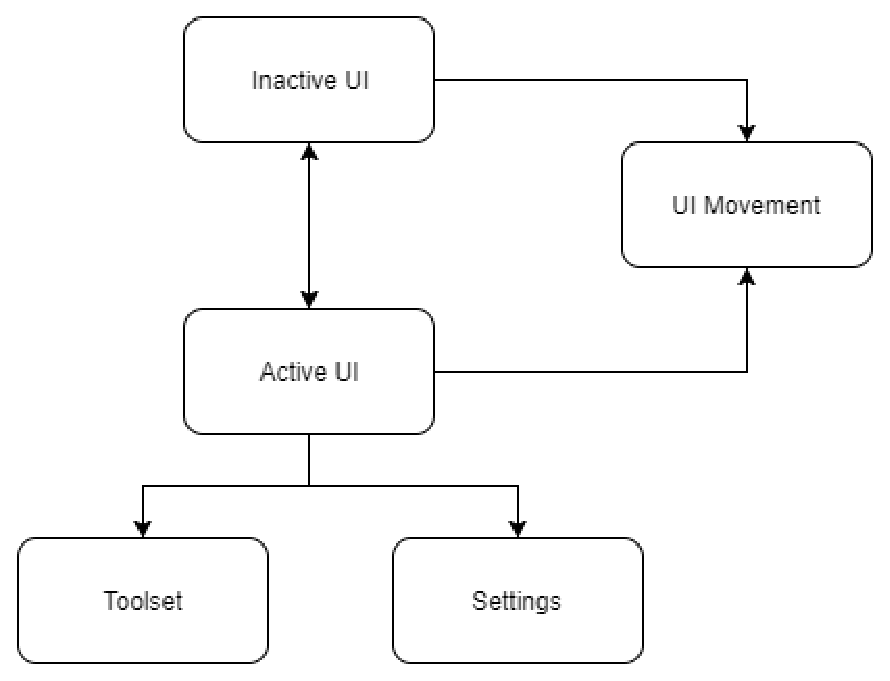
\includegraphics[width=\textwidth]{UIDiagram.eps}
\caption{An example of a tail swap that could be carried out during a balancing procedure}
\end{center}
\end{figure}

\subsection{Architecture of the Interchange}
The Interchange will be the primary point of communication and manager for the disparate elements of the program. The Interchange must be able to receive information supplied via the user interface and interface hardware and relay the corresponding instruction to the Yggdrasil engine to properly render the scene, and is directly responsible for directing state transition of all other components. Due to the experimental nature of the project, the design of the Interchange must be kept at a high level. Specifics of functions and the processing of data will need to be determined in development. 

The Interchange must be capable of properly coordinating all other elements of PolyVox as a whole, and is a central element  in executing commands supplied via user interactions, implementing program features, and directing the graphics engine’s rendering operations. As such it is relevant to design concerns of all stakeholders involved in the project. In particular, it is central to the operation of the user interface and motion controls, from which it will receive user commands, and the operation of the graphics engine, which it will send commands to. As the Interchange will be the point at which the program’s toolset is constructed, it will also dictate the program’s available features.

\subsubsection{Design Entities}
\textbf{Unity Engine:}\\
The Interchange will be built in and run on the Unity Game Engine. Unity has its own proprietary rendering and modeling systems, as well as native compatibility with motion tracking systems and dual rendering used in VR. Additionally, Unity has native scripting compatibility and will serve as the platform for developing the program tools and features.\cite{unity}\\
\textbf{C\#:}\\
C\# is one of the most frequently used languages for scripting in game engines, and is natively compatible with Unity. Most features and tools for the program will be constructed using C\#. 

\subsubsection{Design}
When in operation, the Interchange will receive positional information from the user via both the HMD and VR motion controls in the form of four-element vector positional coordinates. Using Unity’s native VR drivers, the Interchange will translate these coordinates into a position relative to the voxel state.

Additionally, the data received from the user may or may not include a user-input command via a button press. When pressed, the button input will be sent to a function, which is also passed the current state of the UI. This state would include factors such as what ‘brush’ is selected, or what menu the user currently has open. The function will process the user command to determine any possible UI state changes, as well as any changes to the voxel state the user command will perform. 

Any changes in the state are returned by the function as a set of commands to the graphics engine. The graphics engine will then process the commands from the Interchange. Before the render is sent to the HMD, the graphics engine will return a flag that will determine if the Interchange needs to perform additional actions, such as sending a command to the GPU to allocate additional memory. If so, the Interchange will send the appropriate commands, and the graphics engine will reattempt the render. This repeats until the flag sent from the GPU is null. 

While the operations of the Interchange are primarily just in service to other elements of the program, they are still vitally necessary to PolyVox’s operation. The Interchange effectively acts as the driver for the graphics engine and the motion control system, and is needed in order to develop a working feature set and comfortable user interface. See figure 5 for diagram.

\begin{figure}[H]
\begin{center}
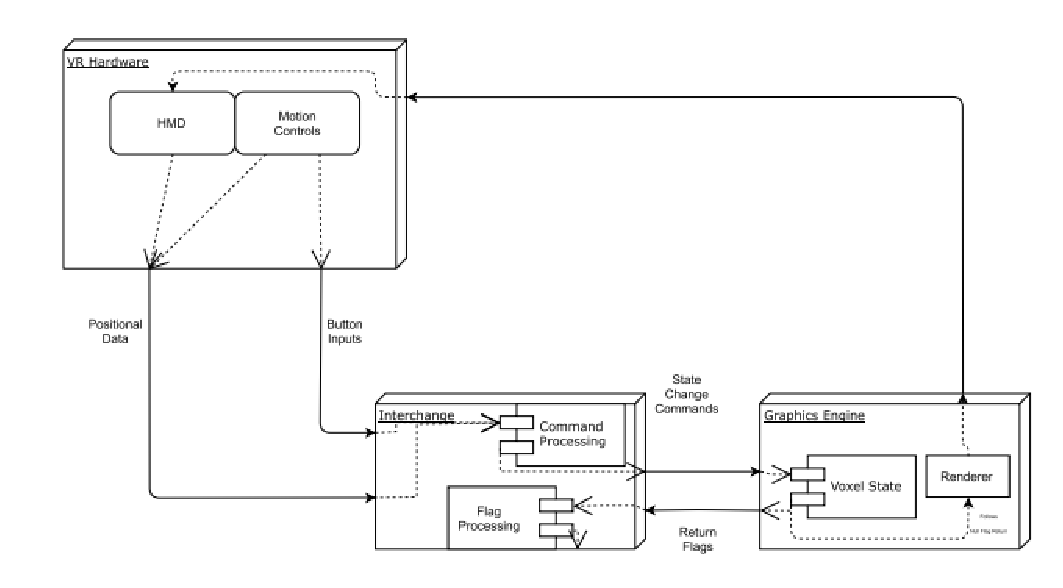
\includegraphics[width=\textwidth]{Interchange.eps}
\caption{General architecture of the Interchange}
\end{center}
\end{figure}
\end{document}
